
% VLDB template version of 2020-08-03 enhances the ACM template, version 1.7.0:
% https://www.acm.org/publications/proceedings-template
% The ACM Latex guide provides further information about the ACM template

\documentclass[sigconf, nonacm, letterpaper,top=2cm,bottom=2cm,left=3cm,right=3cm,marginparwidth=1.75cm]{acmart}

%% The following content must be adapted for the final version
% paper-specific
\newcommand\vldbdoi{XX.XX/XXX.XX}
\newcommand\vldbpages{XXX-XXX}
% issue-specific
\newcommand\vldbvolume{19}
\newcommand\vldbissue{1}
\newcommand\vldbyear{2025}
% should be fine as it is
\newcommand\vldbauthors{\authors}
\newcommand\vldbtitle{\shorttitle} 
% leave empty if no availability url should be set
\newcommand\vldbavailabilityurl{}
% whether page numbers should be shown or not, use 'plain' for review versions, 'empty' for camera ready
\newcommand\vldbpagestyle{plain} 

\usepackage{adjustbox}
\usepackage{pgfplots}
\usetikzlibrary{arrows.meta}
% Useful packages
\usepackage{amsmath}
\usepackage{graphicx}
\usepackage{booktabs}
\usepackage[linesnumbered,ruled,vlined]{algorithm2e}
\SetKw{KwDownTo}{down to}
\begin{document}
\title{A Simple Cache-Sensitive Skip List (SCSSL)}

%%
%% The "author" command and its associated commands are used to define the authors and their affiliations.
\author{Yuchang Ke}
\affiliation{%
  \institution{independent researcher}
  \streetaddress{No. 12, Guandong Street, Hongshan District, Wuhan, Hubei Province.}
  \city{Wuhan}
  \state{China}
  \postcode{430073}
}
\email{aceking.ke@gmail.com}

\author{Bill Lv}
\affiliation{%
  \institution{independent researcher}
  \streetaddress{Phoenix Garden, Optics Ave, Wuhan, Hubei Province}
  \city{Wuhan}
  \state{China}
  \postcode{430073}
}
\email{ideaalloc@gmail.com}

\author{Weijie Zhang}
\affiliation{%
  \institution{Hubei Changjiang Yunxin Media Group Co. Ltd} 
  \streetaddress{No. 788, Gaoxin Ave., Hubei Broadcasting&TV Media Tower,Hubei Province}
  \city{Wuhan}
  \state{China}
  \postcode{430000}
}
\email{zhangweijie@gmail.com}

%%
%% The abstract is a short summary of the work to be presented in the
%% article.
\begin{abstract}
We present a cache-sensitive skip list (SCSSL) that is remarkably simple and easy to implement. It requires only minor modifications to the original skip list data structure to adapt it effectively to modern CPU architectures. This adaptation results in a performance improvement typically ranging from 1.2x to 1.6x, and on some systems, can reach 2x to 3x for insertion-heavy workloads.
Unlike other optimization techniques, SCSSL does not rely on specialized hardware instructions like SIMD or intricate multi-threaded programming paradigms. Instead, its design inherently benefits from improved data locality due to the use of arrays at the data level, a feature that modern compilers can further leverage. This makes the proposed design broadly applicable, suitable not only for in-memory databases and key-value stores but also for resource-constrained embedded systems. and the github is https://github.com/acekingke/simpleCacheSentiveSkiplist
\keywords{skip list; cache-sensitive; index structure; data structures; performance optimization}
\end{abstract}

\maketitle

%%% do not modify the following VLDB block %%
%%% VLDB block start %%%
\pagestyle{\vldbpagestyle}
\begingroup\small\noindent\raggedright\textbf{PVLDB Reference Format:}\\
\vldbauthors. \vldbtitle. PVLDB, \vldbvolume(\vldbissue): \vldbpages, \vldbyear.\\
\href{https://doi.org/\vldbdoi}{doi:\vldbdoi}
\endgroup
\begingroup
\renewcommand\thefootnote{}\footnote{\noindent
This work is licensed under the Creative Commons BY-NC-ND 4.0 International License. Visit \url{https://creativecommons.org/licenses/by-nc-nd/4.0/} to view a copy of this license. For any use beyond those covered by this license, obtain permission by emailing \href{mailto:info@vldb.org}{info@vldb.org}. Copyright is held by the owner/author(s). Publication rights licensed to the VLDB Endowment. \\
\raggedright Proceedings of the VLDB Endowment, Vol. \vldbvolume, No. \vldbissue\ %
ISSN 2150-8097. \\
\href{https://doi.org/\vldbdoi}{doi:\vldbdoi} \\
}\addtocounter{footnote}{-1}\endgroup
%%% VLDB block end %%%

%%% do not modify the following VLDB block %%
%%% VLDB block start %%%
\ifdefempty{\vldbavailabilityurl}{}{
\vspace{.3cm}
\begingroup\small\noindent\raggedright\textbf{PVLDB Artifact Availability:}\\
The source code, data, and/or other artifacts have been made available at \url{\vldbavailabilityurl}.
\endgroup
}
%%% VLDB block end %%%

\section{Introduction}

In computer science, ordered data structures are fundamental for organizing and managing data efficiently. The performance of search, insertion, and deletion operations within these structures is crucial for a wide array of applications, as it directly impacts overall system performance.
Numerous methods have been developed to achieve high performance in ordered data structures, such as AVL trees and Red-Black trees. However, these balanced tree structures are relatively complex to implement due to the necessity of rebalancing operations. This landscape changed when William Pugh introduced the skip list in 1990 \cite{ref1}. The skip list, a probabilistic data structure, offered a simpler implementation alternative to traditional balanced trees while providing comparable performance characteristics.

Thanks to its simplicity and efficiency, the skip list has been widely adopted in various systems. Notable examples include databases like LevelDB \cite{ref2}, Redis \cite{ref7}, RocksDB \cite{ref3} and HBase \cite{ref4}, as well as in-memory caches and the inverted index component of search engines like Lucene.

A standard skip list consists of multiple levels: a data level (level 0) that stores all data nodes in a sorted linked list, and multiple index levels above it. These index levels contain a subset of the nodes from lower levels and act as \textbf{express lanes} to expedite traversal to the desired data nodes. However, nodes in a skip list are typically allocated dynamically, leading to non-contiguous memory addresses. This fragmentation can degrade performance on modern CPUs due to frequent cache misses.

Although ESL, CSSL has developed cache sensitive skip lists to fit modern CPU architecture, these algorithms are still complex, and CSSL uses SIMD instructions which are special in Intel. We strongly believe that the value of a skiplist lies in its simplicity.  Excessively complex cache-sensitive designs reduce the appeal of skip list variations.

Although cache-sensitive skip list variants like the Cache-Sensitive Skip List (CSSL) \cite{ref5} and ESL (Express Lane Skip List) \cite{ref6} have been developed to better align with modern CPU architectures, they often introduce significant complexity. For instance, CSSL utilizes SIMD instructions, which may not be universally available or optimal across all platforms. ESL proposes merging index level nodes into arrays and employs sophisticated version-based locking protocols and lock-free operation logs for concurrency. We believe that the primary appeal of the skip list lies in its inherent simplicity. Overly complex cache-sensitive designs can diminish this advantage.

Our work is motivated by the observation that simple architectural changes can yield substantial performance gains by improving cache locality. We propose a modification that retains the core simplicity of the skip list while significantly enhancing its cache-friendliness.

\section{Design overview}

In this paper, we present a simple and easy-to-implement cache-sensitive skip list. At the data level, it introduces a vector, and the nodes at this level now store arrays instead of single values. Leveraging CPU cache benefits for small arrays to enhance skip list performance. For example, consider a skip list with a vector at the data level; let's suppose the vector's maximum size is 2, as shown in Figure 1. 

In this paper, we present a Simple Cache-Sensitive Skip List (SCSSL). The core idea is to modify the nodes at the data level (level 0) to store a small, sorted array of elements (e.g., key-value pairs or just keys) instead of a single element. This approach leverages CPU cache locality for these small arrays, thereby enhancing performance. For example, Figure \ref{fig:conceptual_scssl} illustrates a conceptual SCSSL where data nodes hold arrays of maximum size 2.


The design of SCSSL hinges on three key principles:
\begin{enumerate}
    \item \textbf{Array-based Data Nodes:} At the data level (level 0), each node contains a sorted array with a fixed maximum length. For integer keys, a maximum length that allows the node to fit well within CPU cache lines (e.g., up to 128 elements, depending on key/value sizes) is chosen.
    \item \textbf{Index Level Pivot:} For navigation through the index levels (levels 1 and above), only the first element (i.e., the smallest key) of the array in a data-level node (or an index node pointing to such an array) is used as the pivot for comparison.
    \item \textbf{Insertion Handling:} The last element (i.e., the largest key) of an array in a data node is primarily considered during insertion operations, particularly when an array is full and a new key needs to be accommodated.
\end{enumerate}

\begin{figure}[htbp]
\centering
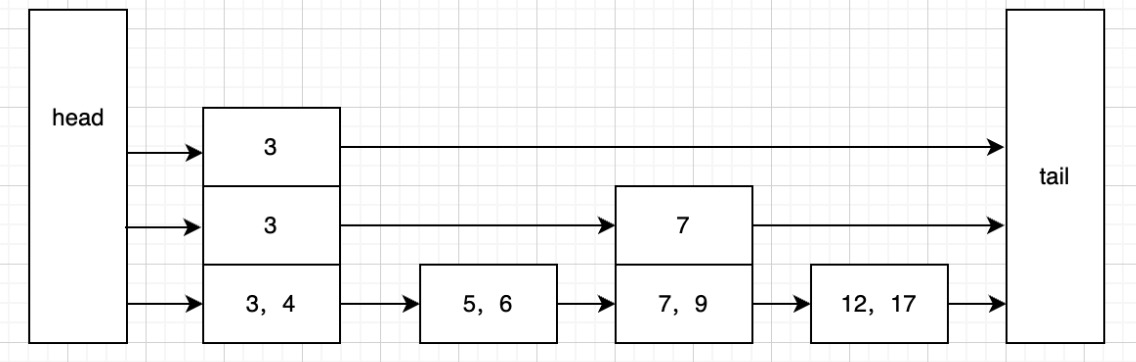
\includegraphics[width=0.7\linewidth]{figures/skiplist.png}
\caption{A conceptual view of the Simple Cache-Sensitive Skip List (SCSSL) where data nodes (level 0) store arrays of elements (e.g., max array size = 2 as depicted). Index nodes point to the start of these arrays.}
\label{fig:conceptual_scssl}
\end{figure}

Our key contributions include:
\begin{enumerate}
    \item Introducing arrays within data-level nodes, which maintains the asymptotic complexity of skip list operations while significantly improving CPU cache hit rates due to the contiguous storage of multiple elements.
    \item Reducing the effective height of the skip list and pointer overhead, as each data-level node now stores multiple elements, leading to fewer nodes overall for a given dataset size.
    \item Presenting modified insertion, search, and deletion algorithms tailored for these array-based data nodes, offering a practical and simple approach for enhancing skip list performance, particularly in database indexing and similar applications.
\end{enumerate}

\section{Algorithm}
This section details the algorithms for search, insertion, and deletion in SCSSL. These operations are adapted from standard skip list algorithms to accommodate the array-based nodes at the data level.

In SCSSL, each node at the data level (level 0) stores its elements in a sorted array of a fixed maximum size. When a new node is created, its level is chosen randomly, similar to a standard skip list. A node promoted to level $k$ has $k+1$ forward pointers (indexed 0 to $k$). The maximum number of levels in the skip list is a predefined constant, \texttt{MAX\_LEVEL}. The skip list employs a header node to initiate searches; its forward pointers are initially Nil. For simplicity in comparisons, the header node can be conceptually considered to hold a key value of negative infinity or have a special marker.
Figure \ref{fig:insertion_example} illustrates an example of an insertion operation in SCSSL.
%uncomment if require: \path (0,302); %set diagram left start at 0, and has height of 302	

\begin{figure}
      \centering
  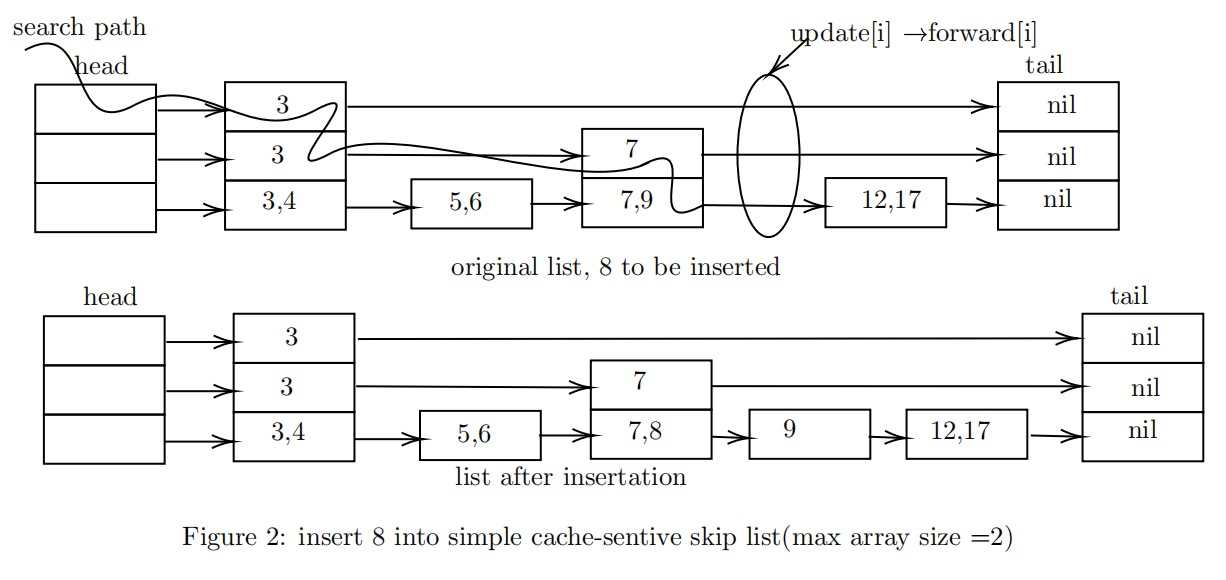
\includegraphics[width=\linewidth]{figures/skipinsert.jpg}
\caption{Insertion of key 8 into an SCSSL (max array size = 2). Key 8 displaces 9 from node (7,9). Key 9 is then inserted into a new node.}
\label{fig:insertion_example}
\end{figure}

\subsection{Initialization}
The initialization process is elementary. A header node is created with an array of \texttt{MAX\_LEVEL+1} forward pointers, all initialized to Nil. To simplify comparisons, the header node's key array (if it were to have one in the same structure) can be considered to contain a single sentinel value of negative infinity, or it can be handled as a special case. In our algorithms, \texttt{header.FirstKey()} would effectively be $\infty$.


\subsection{Search}
\begin{algorithm}
    \caption{Search Key in simple cache-sentive skip list}
    \KwIn{Key $k$}
    \KwOut{Node containing key or Nil}
    \SetKwFunction{FMain}{search}
    \SetKwProg{Fn}{Function}{:}{}
    \Fn{\FMain{$k$}}{
        $current \gets header$\;
        
        \For{$i \gets level$ \KwDownTo $0$}{
            \While{$current.forward[i] \neq \text{Nil} \land current.forward[i].Key() \leq k$}{
                $current \gets current.forward[i]$\;
            }
        }
        
        \KwRet{$current.search\_in\_array(k)$}\;
    }
\end{algorithm}

As the algorithm shows in Algorithm 1, from line 3 to line 5, it’s very similar to a standard skip list, but in line 4,current.forward[i].Key() returns the least value(at the first position) of the array in the \texttt{current.forward[i]}. Out of the while loop, the current’s forward Key() must be just greater than key, and if the key exists in the data structure, it must be in the current node array, so just search in the array of the current node in line 6.


\subsection{Insertion}
\begin{algorithm}
    \caption{Insert Key into simple cache-sentive skip list}
    \KwIn{Key $k$}
    \KwOut{Nil}
    \SetKwFunction{FMain}{insert}
    \SetKwProg{Fn}{Function}{:}{}
    \Fn{\FMain{$k$}}{
        $update \gets \text{array of size } (max\_level + 1)$\;
        $current \gets header$\;
        
        \For{$i \gets \texttt{level}$ \KwDownTo $0$}{
            \While{$current.forward[i] \neq \text{Nil} \land current.forward[i].Key() \leq k$}{
                $current \gets current.forward[i]$\;
            }
            $update[i] \gets current$\;
        }
        
        \If{$current \neq header \land current.is\_full() \land current.array[-1] > k$}{
            $replace \gets current.array.pop()$\;
            $current.insert\_into\_array(k)$\; \tcp{CASE 1}
            $k \gets replace$\;
        }
        
        \If{$current \neq header \land \neg current.is\_full()$}{ \tcp{CASE 2}
            $current.insert\_into\_array(k)$\;
        }
        \Else{ \tcp{CASE 3}
            $current \gets current.forward[0]$\;
            \If{$current \neq \text{Nil} \land current \neq header \land \neg current.is\_full()$}{
                $current.insert\_into\_array(k)$\;
                \KwRet{}
            }
            
            $new\_level \gets random\_level()$\;
            
            \If{$new\_level > level$}{
                \For{$i \gets level + 1 \KwDownTo new\_level$}{
                    $update[i] \gets header$\;
                }
                $level \gets new\_level$\;
            }
            
            $new\_node \gets Node([k], new\_level)$\;
            
            \For{$i \gets 0 $ \KwTo $new\_level$}{
                $new\_node.forward[i] \gets update[i].forward[i]$\;
                $update[i].forward[i] \gets new\_node$\;
            }
        }
    }
\end{algorithm}
In Algorithm 2, from line 2 to line 7, it’s the same as a standard skip list. However, from line 8 to line 18, It should consider that level 0 nodes have a array. So there are several constraints which cannot be ignored:

\begin{itemize}


\item  If the current node is a header, a new node should be created to insert the key. We don’t want to insert data in the header; otherwise, it will be trouble for the deletion operation. So, in line 8-18, we exclude the header.
  
There are some cases for insertion:

\item CASE 1: current is not header, but current array size reach the maximum size(\texttt{current.is\_full()} function to check it) and key value is between the least element (first position, Key() return it) and the largest element(last position, \texttt{current.array[-1]}). So in this case, current node’s array is full, we make a small strick to deal with it, we pop the last position element, so the array is not full, and we insert the key in current node array(line 9,10) and it must be full again.then go on the next steps(for example, we replace 9 with 8 , and then insert 9 in another node, see Figure 2).

\item CASE 2: current is not header, current node’s array is not full, just insert the key in the array(line 12, 13). Then the insertion operation is finished.

\item CASE 3: The key is lower than current.forward’s the least value of its array(lines 4-7 has insurance for this), and the key is greater than the largest element of current node’s array, So this key should be inserted into the current’s forward node. We just insert it when the node is not full (from line 15-18), and we do not pop last element like line 9-11, for just to be simple.
\item Other CASES:  we should create a new node and insert the key in its array , and modify the forward pointers(from line 19 to 27)
\end{itemize}

\subsection{Deletion}

\begin{algorithm}
        \caption{Delete key from simple cache-sentive skip list}
        \KwIn{Key $k$}
        \KwOut{True if deleted, False otherwise}
        \SetKwFunction{FMain}{delete}
        \SetKwProg{Fn}{Function}{:}{}
        \Fn{\FMain{$k$}}{
            $update \gets \text{array of size } (max\_level + 1)$\;
            $current \gets header$\;
            
            \For{$i \gets level$ \KwDownTo $0$}{
                \While{$current.forward[i] \neq \text{Nil} \land current.forward[i].array[-1] < k$}{
                    $current \gets current.forward[i]$\;
                }
                $update[i] \gets current$\;
            }
            
            $current \gets current.forward[0]$\;
            \If{$current = \text{Nil}$}{
                \KwRet{False}\;
            }
            \Else{
                $res \gets current.delete\_from\_array(k)$\;
                \If{$\neg res$}{
                    \KwRet{False}\;
                }
            }
            
            \If{$\text{len}(current.array) = 0$}{
                \For{$i \gets$ 0 $\KwTo$ $level$}{
                    \If{$update[i].forward[i] \neq current$}{
                        \textbf{break}; % Use KwBreak instead of Break
                    }
                    $update[i].forward[i] \gets current.forward[i]$\;
                }
                
                \While{$level > 0 \land header.forward[level] = \text{Nil}$}{
                    $level \gets level - 1$\;
                }
                \KwRet{True}\;
            }
        }
\end{algorithm}
    



The deletion algorithm is shown in Algorithm 3, which should be noted that in line 5,  the condition checks whether the current forward array's largest element is less than k, so out of the while loop,  \texttt{current.forward[0]} is the first node whose largest element is equal to or greater than k, which means that if the key exists, it must be in the current node’s \texttt{forward[0]} array. Line 8 to 14, delete the key in the selected array, and Line 15 to 21 checks whether the array is empty, if it is empty, we should delete the node from the data structure.


\section{Evaluation}
\subsection{Experimental Environment}

The experiments were conducted in the following environments:
\begin{itemize}
    \item \textbf{Hardware 1 (MacBook):} Apple M2 CPU, 16 GB RAM.
    \item \textbf{Hardware 2 (Server):} Intel(R) Core(TM) i7-6700 CPU @ 3.40GHz, 24 GB DDR4 2133 MHz RAM. This server was used not only for performance testing but also specifically for analyzing CPU cache miss rates using appropriate profiling tools (e.g.,  \texttt{perf} ).
    \item \textbf{Compiler:} The algorithms were implemented in C++. The test programs were compiled using g++ (version specific to environment, e.g., 9.0 or higher) with the \texttt{-O3} optimization flag.
    \item \textbf{Benchmark Configuration:}
        Insertion operations in a skip list are prone to CPU cache misses due to dynamic memory allocations and pointer chasing. Therefore, our benchmarks primarily focus on insertion performance using randomly generated integer keys. The number of elements ranged from 100 to 300,000.
        Search performance was also evaluated. However, we do not present detailed search results as the performance difference between SCSSL and the standard skip list was found to be negligible for typical search operations. This is likely because the dominant factor in search is the traversal of levels, which has a similar path length, and the final array scan in SCSSL is very fast for small arrays.
        Both the standard skip list and SCSSL were configured with a maximum level (MAX\_LEVEL) of 16. For SCSSL, the maximum array size within a data node was set to a value empirically found to be effective (e.g., 64 or 128, chosen to fit well within L1 cache lines).
\end{itemize}


\subsection{Results and Discussion}
\begin{figure}
\centering
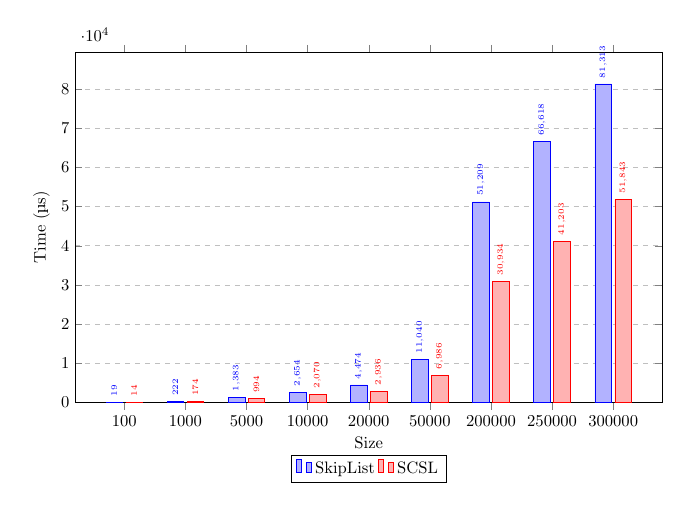
\begin{tikzpicture}[scale=0.6]
\begin{axis}[
    ybar,
    bar width=10pt,
    width=14cm,
    height=9cm,
    enlarge x limits=0.1,
    xlabel={Size},
    ylabel={Time (µs)},
    symbolic x coords={100,1000,5000,10000,20000,50000,200000,250000,300000},
    xtick=data,
    legend style={at={(0.5,-0.15)},anchor=north,legend columns=2},
    nodes near coords,
    every node near coord/.append style={font=\tiny, rotate=90, anchor=west},
    ymin=0,
    ymajorgrids=true,
    grid style=dashed
]
\addplot+[style={blue,fill=blue!30}] coordinates {
    (100,19) (1000,222) (5000,1383) (10000,2654)  (20000,4474) (50000,11040) (200000,51209) (250000,66618) (300000,81313)
};
\addplot+[style={red,fill=red!30}] coordinates {
    (100,14) (1000,174) (5000,994) (10000,2070)  (20000,2936) (50000,6986) (200000,30934) (250000,41203) (300000,51843)
};

\legend{SkipList, SCSL}
\end{axis}
\end{tikzpicture}
\caption{Insertion Time Comparison Between SkipList and SCSL at Different Scales(smaller is better) in Macos}
\end{figure}

\begin{figure}
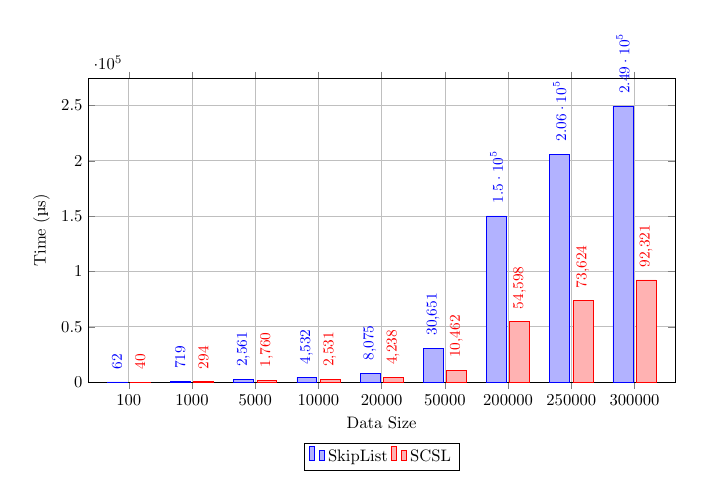
\begin{tikzpicture}[scale=0.6]
\begin{axis}[
    width=14cm,
    height=8cm,
    ybar,
    bar width=12pt,
    symbolic x coords={100,1000,5000,10000,20000,50000,200000,250000,300000},
    xtick=data,
    xlabel={Data Size},
    ylabel={Time (µs)},
    legend style={at={(0.5,-0.2)},anchor=north,legend columns=-1},
    enlarge x limits=0.08,
    ymin=0,
    grid=major,
    nodes near coords,
    nodes near coords style={font=\small, anchor=west, rotate=90, xshift=4pt},
]

\addplot coordinates {(100,62) (1000,719) (5000,2561) (10000,4532) (20000,8075) (50000,30651) (200000,150126) (250000,206036) (300000,249135)};
\addplot coordinates {(100,40) (1000,294) (5000,1760) (10000,2531) (20000,4238) (50000,10462) (200000,54598) (250000,73624) (300000,92321)};

\legend{SkipList, SCSL}
\end{axis}
\end{tikzpicture}
\caption{Insertion Time Comparison Between SkipList and SCSL at Different Scales(smaller is better) in Server}
\end{figure}


\begin{table*}[t]
\begin{tabular}{lrrr}
\toprule
Test Case & Cache References & Cache Misses & Cache Misses Rate \\
\midrule
\verb|SCSL| & 51,567,218 & 459,636 & 0.89\% \\
\verb|Standard Skip List| & 142,249,678 & 47,251,323 & 33.22\% \\
\bottomrule
\end{tabular}
\caption{Cache Performance Comparison Between SCSL and standard Skip list in server computer}
\end{table*}


On the MacBook (Apple M2 processor, Figure 3 SCSSL demonstrates a speedup of 1.28x-1.39x for small datasets (<1,000 elements) during insertion. For medium-scale datasets (>20,000 elements), the speedup increases to a range of 1.55x-1.65x. This trend indicates that the cache-friendly benefits of SCSSL become more pronounced as the dataset size grows, leading to more memory accesses.

On the server system (Intel i7-6700, Figure 4, SCSSL achieves even more significant speedups for insertions, reaching up to nearly 3x compared to the standard skip list for larger datasets (e.g., 300,000 elements). This enhanced improvement on the server platform might be attributed to differences in cache architecture, memory subsystem performance, or the relative cost of cache misses compared to the M2 architecture.




Table 1 presents the cache performance data for inserting 300,000 random elements on the server. The standard skip list exhibits a high L1 data cache miss rate of 33.22\%. In contrast, SCSSL drastically reduces this rate to a mere 0.89\%. This substantial reduction in cache misses directly corroborates our hypothesis that embedding arrays within data nodes effectively improves data locality and cache utilization, which translates into the observed speedups. The significantly lower number of cache references for SCSSL also suggests more efficient data access patterns.



\section{Conclusions}

We have presented SCSSL, a novel cache-sensitive skip list variant that introduces a simple yet highly effective modification: replacing single elements in data-level nodes with small, sorted arrays. This architectural change allows SCSSL to enhance CPU cache performance by improving data locality, while crucially maintaining the algorithmic simplicity that is a hallmark of skip lists.

Experimental results demonstrate significant performance improvements for insertion operations, particularly on systems where cache performance is a critical factor. The observed speedups of 1.2x-3x, coupled with a dramatic reduction in cache miss rates (e.g., from 33.22\% to 0.89\% in our server tests), validate the efficacy of this approach. SCSSL offers a practical and easily implementable method to boost skip list performance in modern computing environments without resorting to complex algorithmic changes or specialized hardware features. Its simplicity makes it an attractive option for a wide range of applications, from embedded systems to large-scale in-memory data stores.

Future work could explore optimal array sizes for different hardware platforms and key/value types, as well as investigate the application of SCSSL principles in concurrent skip list implementations.

\begin{thebibliography}{9} 
\bibitem{ref1}
      Skip Lists: A Probabilistic Alternative to Balanced Trees
\bibitem{ref2}
      Google. LevelDB. Available online: https://github.com/google/leveldb (accessed on 20 July 2023).
\bibitem{ref3}
      Facebook. RocksDB. Available online: http://rocksdb.org/ (accessed on 20 July 2023).
\bibitem{ref4}
      Apache. Welcome to Apache HBase™. Available online: https://hbase.apache.org/ (accessed on 20 July 2023).
\bibitem{ref5}
      Cache-Sensitive Skip List: Efficient Range Queries on modern CPUs - informatik.hu-berlin.de.
\bibitem{ref6}
      ESL: A High-Performance Skiplist with Express Lane  https://www.mdpi.com/2076-3417/13/17/9925
\bibitem{ref7}
	Redis, Accessed: 2024-01-09.
\end{thebibliography}
\end{document}